%%%%%%%%%%%%%%%%%%%%%%%%%%%%%%%%%%%%%%%%%%%%%%%%%%%%%%%%%%%%%%%%%%%%%%%%%%%%%%%%%%
%%%%%%%%%%%%%%%%%%%%%%%%%%%%%%%%%%%%%%%%%%%%%%%%%%%%%%%%%%%%%%%%%%%%%%%%%%%%%%%%%%
\section{Introduction}
%%%%%%%%%%%%%%%%%%%%%%%%%%%%%%%%%%%%%%%%%%%%%%%%%%%%%%%%%%%%%%%%%%%%%%%%%%%%%%%%%%
%%%%%%%%%%%%%%%%%%%%%%%%%%%%%%%%%%%%%%%%%%%%%%%%%%%%%%%%%%%%%%%%%%%%%%%%%%%%%%%%%%

We present a Diffusion Synthetic Acceleration (DSA) scheme
that is fully compatible with the Piece-Wise Linear Discontinuous (PWLD) finite
element discretization of the transport equation on arbitrary
polygonal cells. 

Arbitrary polygonal (polyhedral in 3D) cells can advantageously employed, especially
in the context of spatial discretizations based on discontinuous finite elements (DFE).
Such grids may allow for a reduced numbers of unknowns and/or can provide a natural
transition for locally adapted meshes. To illustrate these two points, first consider
a hexagonal cell. Employing a PWLD discretization, such cell possesses six unknowns. Using
alternate DFE discretizations that perform well in the thick diffusive limit, such as 
linear discontinuous on triangles and bilinear discontinuous on quadrangles, the same 
hexagonal cell could be split into two quadrangles (for a total of 8 unknowns), two 
triangles and one quadrangle (10 unknowns), four triangles (12 unknowns); by inserting an 
extra point inside the cell, the hexagon could also be split into three quadrangles 
(12 unknowns), four quadrangles (16 unknowns) or six triangles (18 unknowns). A 
similar reasoning can be applied to any $n$-polygon. Arbitrary polygonal grids can 
also handle locally refined meshes in a natural manner. Consider the example given
in \Cref{fig_amr}, which is typical of simulations performed with Adaptive Mesh 
Refinement. Solvers based on arbitrary polyhedral cells can easily handle cells 
with various numbers of edges. On \Cref{fig_amr}, the left cell is a actually a
pentagon whereas the two cells on the right are quadrilaterals. PWLD spatial
discretization can handle locally adapted meshes without any special treatment 
or further approximation of the coupling between cells.
\begin{figure}[H]
   \centering
   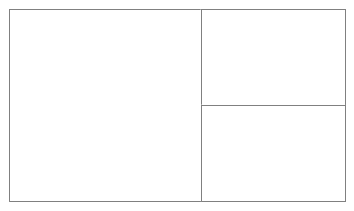
\includegraphics[width=0.3\textwidth]{amr}
   \caption{AMR mesh.}
   \label{fig_amr}
\end{figure}


%%%%%%%%%%%%%%%%%%%%%%%%%%%%%%%%%%%%%%%%%%%%%%%%%%%%%%%%%%%%%%%%%%%%%%%%%%%%%%%%%%
%\subsection{Rationale for DSA preconditioning}
%%%%%%%%%%%%%%%%%%%%%%%%%%%%%%%%%%%%%%%%%%%%%%%%%%%%%%%%%%%%%%%%%%%%%%%%%%%%%%%%%%

Next, we first recall the rationale for acceleration schemes (preconditioners) 
\textcolor{red}{applied to the iterative solution of
transport problems / when solving iteratively transport problems.}
Because analytical solutions are unavailable for most
radiation transport problems of practical interest, one typically employs
iterative techniques to solve the large system of equations that results from
the spatial and angular discretizations of the transport equation. Standard
iterative techniques for the first-order form of the discrete-ordinate (\sn)
transport equation include the Source Iteration (SI) technique and Krylov 
subspace algorithms (usually GMRes \cite{gmres}). For highly diffusive materials 
(i.e., with scattering ratios $c=\Sigma_s / \Sigma_t $ close to 1) and optically 
thick configurations (i.e., problems that are not leakage-dominated), these iterative techniques 
can become quite ineffective, requiring high iteration counts and possibly 
leading to false convergence. To mitigate these issues, SI and GMRES-based transport solves 
can be effectively accelerated (preconditioned) using DSA approaches 
\cite{dsa_ref,larsen_dsa,consistent_p1,m4s,wla,mip}. 

The spatial discretization of the DSA equations
must be somewhat ``consistent'' with the one used for the \sn transport equations 
in order to yield unconditionally stable and efficient DSA schemes
\cite{dsa_ref,larsen_dsa,consistent_p1,m4s,wla,mip}. However, the search for full
consistency between the discretized transport equations and the discretized
diffusion may not be computationally practical (especially for unstructured
arbitrary meshes, \cite{dsa_ref}). For instance, Warsa, Wareing, and
Morel \cite{consistent_p1} derived a fully consistent DSA scheme for linear
discontinuous finite elements on unstructured tetrahedral meshes; their DSA
scheme yielded in a $P_1$ system of equations which was found to be
computationally more expensive than partially consistent DSA schemes that are
based upon discretizations of a standard diffusion equation. Some partially 
consistent schemes have been analyzed for discontinuous finite element
(DFE) discretizations of the transport equation on unstructured meshes, for
example, the modified-four-step (M4S) scheme \cite{m4s}, the
Wareing-Larsen-Adams (WLA) scheme \cite{wla}, and the Modified Interior
Penalty (MIP) scheme \cite{mip}.

%%%%%%%%%%%%%%%%%%%%%%%%%%%%%%%%%%%%%%%%%%%%%%%%%%%%%%%%%%%%%%%%%%%%%%%%%%%%%%%%%%
%\subsection{PWLD discretization on arbitrary grids}
%%%%%%%%%%%%%%%%%%%%%%%%%%%%%%%%%%%%%%%%%%%%%%%%%%%%%%%%%%%%%%%%%%%%%%%%%%%%%%%%%%

%% Several discretization methods haven been developed for 
%% arbitrary polygonal meshes \cite{pwld_2d,pwld_3d,cfm_dfm,pwl_diffusion,
%% palmer_fe,mimetic,cell_centered_diff,palmer_proc,palmer_ane,wachspress,pwbld}.
%% In this work, we focus on the PWLD discretization because it was successfully
%% used to discretize the transport equation \cite{pwld_2d,pwld_3d}. This
%% discretization can be applied for any polygonal cells and the integrals
%% generated by this discretization can be easily computed analytically. 

To the authors' best knowledge, no work is currently done to adapt the M4S 
technique to polygonal meshes. This is probably due to the fact
that M4S does not yield a Symmetric Positive Definite (SPD)
matrix and was found to be divergent for 3D tetrahedral meshes with linear 
discontinuous elements. 
% 
Recent work to develop a DSA scheme for polygonal cells has mainly focused 
on adapting the WLA scheme to polygonal meshes
\cite{cfm_dfm,wla_pwl}. The WLA scheme is a two-stage process, where first a
diffusion solution is obtained using a {\em continuous} finite element
discretization and then a {\em discontinuous } update is performed cell-by-cell 
in order to provide an appropriate discontinuous scalar flux correction to the DFE transport 
solver. In \cite{consistent_p1}, the WLA scheme was
found to be a stable and effective DSA technique, though its efficiency
degraded as the problem became more optically thick and highly diffusive.
%
In this paper, we present an extension of the MIP technique to the
PWLD discretization technique for arbitrary polygonal meshes.
The MIP scheme is based on the standard Interior Penalty (IP) method for the
discontinuous discretization of diffusion equations. MIP was first derived in
\cite{mip}, where it was applied to triangular unstructured meshes (with
locally adapted cells). MIP did \textcolor{red}{not suffer from the same problems than WLA when the
problem becomes optically thick and highly diffusive} and it is therefore an
interesting alternative to WLA. Because MIP produces an SPD matrix, it has been 
solved using a Preconditioned Conjugate Gradient (PCG), with symmetric successive 
over-relaxation method (SSOR) as preconditioner \cite{mip}. Here, 
the effectiveness of algebraic multigrid methods (AMG) to precondition the diffusion
solver \cite{amg,amg_course} will be tested and compared with PCG+\textcolor{red}{SGS}.
%Algebraic multigrid methods allow the use of multigrid techniques when no grid
%information is available or when the grid is unstructured. Instead of using a
%succession of grids based on the geometry of the problems, the ``grid levels''
%are based on properties of the matrix.

The remainder of this paper is organized as follows. In \Cref{sec_transport},
we briefly recall the \sn transport equation, its discontinuous finite element
discretization using the PWLD technique, and the Source Iteration iterative scheme. 
The MIP scheme is reviewed and extended to the PWLD discretization for arbitrary 
polygons in \Cref{sec_mip}. In \Cref{sec_amg}, we introduce the Algebraic MultiGrid (AMG) 
approaches used here: the ML package of Trilinos \cite{ml_guide} and the
AGMG (AGgregation-based algebraic MultiGrid) technique \cite{agmg_guide}. In
\Cref{sec_res}, we present a Fourier analysis for the MIP scheme discretized with
PWLD and we compare the different AMG with preconditioned CG solver.
Conclusions are given in \Cref{sec_conc}.
